\documentclass[conference]{IEEEtran}
\usepackage{shared/template_tgir_article}
\usepackage{booktabs}
\usepackage{longtable}
\usepackage{tabularx}
\usepackage{array}
\usepackage{enumitem}
\usepackage{xcolor}
\usepackage{listings}

\lstset{
    basicstyle=\ttfamily\small,
    breaklines=true,
    columns=fullflexible,
    frame=single
}

\newcommand{\product}{TGIR QuantLib Tools}
\newcommand{\code}[1]{\texttt{#1}}
\newcommand{\docdate}{2026-04-06}

% Visual design is controlled exclusively by template_tgir_article.sty and
% IEEEtran. Keep this file limited to content-support packages and commands.

\usepackage{amsmath}
\usepackage{lipsum}
\usepackage{tikz}
\usetikzlibrary{arrows.meta,positioning}

\title{Sample TGIR Article: A Reproducible Dummy Research Note}
\TGIRSetArticlePublicationDate{August 30, 2026}
\author{\TGIRArticleAuthorBlock}

\begin{document}
\maketitle

\begin{abstract}
This three-page specimen demonstrates the canonical TGIR article template with
dummy prose, equations, a table, and a content-level diagram. It is not a
research conclusion. Its purpose is to make the expected IEEE-derived format
immediately visible while leaving typography, columns, title treatment, logo,
links, and page numbering under shared-template control.
\end{abstract}

\begin{IEEEkeywords}
dummy research, reproducibility, sample document, validation workflow
\end{IEEEkeywords}

\section{Purpose and Dummy Setting}

Consider a fictional research process that converts a dated input vector
$x_t$ into a reviewable decision score $s_t$. The content in this document is
intentionally illustrative: names, values, and conclusions are placeholders
for a real study. The layout, however, is the production layout that TGIR
working papers use before any venue-specific submission mode is selected.

\lipsum[1]

The sample distinguishes a reproducible method from an attractive narrative.
For each observation, the analyst records an input set, a transformation, an
independent check, and a concise limitation. This sequence keeps the document
useful even when the dummy values are replaced by real measurements.

\begin{equation}
  s_t = \alpha + \beta x_t + \gamma \log(1 + |x_t|) + \varepsilon_t,
  \qquad \varepsilon_t \sim \mathcal{N}(0, \sigma^2).
  \label{eq:dummy-score}
\end{equation}

Equation~\eqref{eq:dummy-score} is deliberately simple. In a real paper,
$\alpha$, $\beta$, $\gamma$, and $\sigma$ would be estimated from a dated,
versioned data set, and the model specification would explain why that choice
is appropriate for the decision at hand.

\begin{table}[!t]
  \caption{Illustrative inputs for the dummy research note}
  \label{tab:dummy-inputs}
  \centering
  \begin{tabular}{lrrl}
    \toprule
    Observation & $x_t$ & $s_t$ & Review state \\
    \midrule
    A & 0.42 & 0.38 & Reconciled \\
    B & 0.67 & 0.61 & Reconciled \\
    C & 0.91 & 0.79 & Sensitivity check \\
    D & 1.08 & 0.90 & Escalated \\
    \bottomrule
  \end{tabular}
\end{table}

\section{Method and Control Logic}

\lipsum[2]

The transformation is evaluated together with a control residual,
\begin{equation}
  r_t = y_t - \widehat{y}_t,
  \qquad
  \operatorname{RMSE} =
  \sqrt{\frac{1}{T}\sum_{t=1}^{T} r_t^2}.
  \label{eq:dummy-rmse}
\end{equation}
where $y_t$ is a fictional benchmark and $\widehat{y}_t$ is the model output.
The residual is not merely reported; it determines whether the evidence can
support circulation, requires a documented limitation, or must be reworked.

\begin{figure}[!t]
  \centering
  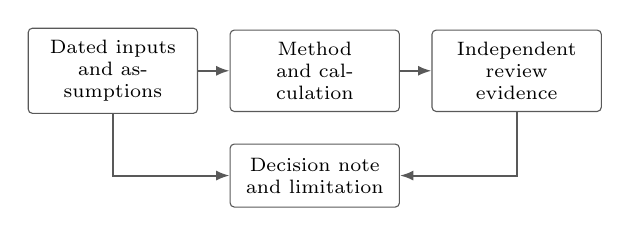
\begin{tikzpicture}[
    node distance=4mm,
    every node/.style={font=\scriptsize},
    box/.style={draw=black!65, rounded corners=1.5pt, align=center,
      minimum height=8mm, text width=1.85cm, inner sep=1.5mm},
    flow/.style={-{Latex[length=1.7mm]}, line width=.7pt, draw=black!65}
  ]
    \node[box] (inputs) {Dated inputs\\and assumptions};
    \node[box, right=of inputs] (model) {Method\\and calculation};
    \node[box, right=of model] (review) {Independent\\review evidence};
    \node[box, below=of model] (decision) {Decision note\\and limitation};
    \draw[flow] (inputs) -- (model);
    \draw[flow] (model) -- (review);
    \draw[flow] (review) |- (decision);
    \draw[flow] (inputs) |- (decision);
  \end{tikzpicture}
  \caption{A content-level dummy workflow. The shared template, not this
  diagram, determines the document's overall visual style.}
  \label{fig:dummy-workflow}
\end{figure}

Figure~\ref{fig:dummy-workflow} shows the minimum evidence path. The diagram
is intentionally local to the subject matter: it does not redefine page
geometry, headings, colors, title formatting, or any other template behavior.

\section{Illustrative Results}

\lipsum[3-5]

Table~\ref{tab:dummy-results} presents invented result categories. The table
is here to demonstrate alignment, caption treatment, and numeric structure;
it should never be interpreted as a recommendation.

\begin{table}[!t]
  \caption{Illustrative dummy result categories}
  \label{tab:dummy-results}
  \centering
  \begin{tabular}{lrr}
    \toprule
    Scenario & Dummy estimate & Check difference \\
    \midrule
    Base case & 101.2 & 0.0 \\
    Mild stress & 98.7 & -2.5 \\
    Severe stress & 93.4 & -7.8 \\
    Independent benchmark & 100.9 & -0.3 \\
    \bottomrule
  \end{tabular}
\end{table}

For the dummy base case, a threshold rule can be written as
\begin{equation}
  d_t =
  \begin{cases}
    \text{circulate}, & |r_t| \leq \tau_1, \\
    \text{qualify}, & \tau_1 < |r_t| \leq \tau_2, \\
    \text{escalate}, & |r_t| > \tau_2,
  \end{cases}
  \label{eq:dummy-threshold}
\end{equation}
where $\tau_1$ and $\tau_2$ are review thresholds fixed before the result is
observed. A real implementation would also retain the input hash, code version,
reviewer identity, and timestamp that produced each decision state.

\section{Validation and Limitations}

\lipsum[6-8]

The practical validation checklist is short. First, reconcile the underlying
inputs to their dated sources. Second, reproduce the calculation from a clean
environment. Third, compare output to an independent benchmark. Finally,
describe the most consequential limitation in plain language before a reader
uses the work. These steps are deliberately more important than increasing the
visual decoration of a sample document.

\lipsum[10-13]

\lipsum[14-17]

\section{Conclusion}

\lipsum[9]

This dummy note has shown the canonical TGIR article format across three pages:
an IEEE-derived two-column layout, restrained first-page branding, publication
date, page numbers, mathematical notation, tables, and a content-level diagram.
Replace the dummy material with actual evidence while retaining the shared
template import and avoiding document-level style overrides.

\end{document}
